\documentclass[../main.tex]{subfiles}

\graphicspath{{../images/}}

\begin{document}
\pagestyle{fancy}
\lhead{Homework 7}
\chead{Junseo Shin}
\rhead{PHYS 421}

\setcounter{section}{7}

% 4.15, 4.17, 4.19, 4.37
\paragraph{4.15} Thick spherical shell of inner radius $a$, outer radius $b$, with polarization
\begin{align*}
    \vb P (\vb r) = \frac{k}{r} \vu r    
\end{align*}
\begin{itemize}
    \item [(a)] E-field in all regions using bound charges: The volume bound charge is
    \begin{align*}
        \rho_b &= -\div \vb P = - \frac{1}{r^2} \pdv{r}(r^2 \frac{k}{r}) = -\frac{k}{r^2}
    \end{align*}
    and the surface bound charges are ($\vu n = -\vu r$ at $r = a$)
    \begin{align*}
        \sigma_b = \vb P \vdot \vu n = \begin{cases}
            -\dfrac{k}{a} & r = a \\
            \dfrac{k}{b} & r = b
        \end{cases}
    \end{align*}
    Using Gauss's Law
    \begin{align*}
        \oint \vb E \vdot \dd \vb a &= \frac{Q_\text{enc}}{\epsilon_0}
    \end{align*}
    \begin{itemize}
        \item [(i)] $r < a$: $Q_\text{enc} = 0$, so $\vb E = 0$
        \item [(ii)] $a < r < b$: The enclosed charge is the inner surface charge plus the volume charge:
        \begin{align*}
            Q_\text{enc} &= \oint_S \sigma_b \dd{\vb a} + \int_V \rho_b \dd{\tau} \\
            &= \int -\frac{k}{a} a^2 \sin\theta \dd{\theta} \dd{\phi} + \int -\frac{k}{r^2} r^2 \sin\theta \dd{r} \dd{\theta} \dd{\phi} \\
            &= -4\pi k a - 4\pi k (r - a) = -4\pi k r
        \end{align*}
        So using Gauss's Law
        \begin{align*}
            \oint \vb E \vdot \dd{\vb a} &= \frac{Q_\text{enc}}{\epsilon_0} \\
            \abs{\vb E} \oint \dd{a} &= -\frac{4\pi k r}{\epsilon_0} \\
            \abs{\vb E} 4\pi r^2 &= -\frac{4\pi k r}{\epsilon_0} \\
            \abs{\vb E} &= -\frac{k}{\epsilon_0 r} 
        \end{align*}
        or 
        \begin{align*}
            \vb E = -\frac{k}{\epsilon_0 r} \vu r
        \end{align*}
        \item [(iii)] $r > b$: The total enclosed charge of a dielectric is zero (from last HW 4.14), so $\vb E = 0$
    \end{itemize}
    \item [(b)] Using
    \begin{align*} \tag{4.23}\label{eq:4.23}
        \oint D \vdot \dd{\vb a} = Q_\text{free}
    \end{align*}
    and 
    \begin{align*} \tag{4.21} \label{eq:4.21}
        \vb D = \epsilon_0 \vb E + \vb P
    \end{align*}
    the total free enclosed charge is zero, so
    \begin{align*}
        \vb D = 0
    \end{align*}
    Thus
    \begin{align*}
        \epsilon_0 \vb E + \vb P = 0 
    \end{align*}
    or
    \begin{align*}
        \vb E = -\frac{1}{\epsilon_0} \vb P = \begin{cases}
            0 & r < a \qand r > b \\
            -\dfrac{k}{\epsilon_0 r} \vu r & a < r < b
        \end{cases}
    \end{align*}
\end{itemize}

\newpage
\paragraph{4.17} Bar electret from Prob. 4.11 has $\rho_b = 0$: From divergence theorem
\begin{align*}\tag{4.22}
    \int_V (\div \vb D) \dd{\tau} = \oint_S \vb D \vdot \dd{\vb a} = Q_\text{free} = 0 \implies \div \vb D = 0
\end{align*}
So, the field lines for $\vb D$ are closed loops as shown in Fig. \ref{fig:hw7_1}.

\begin{figure*}[ht]
    \centering
    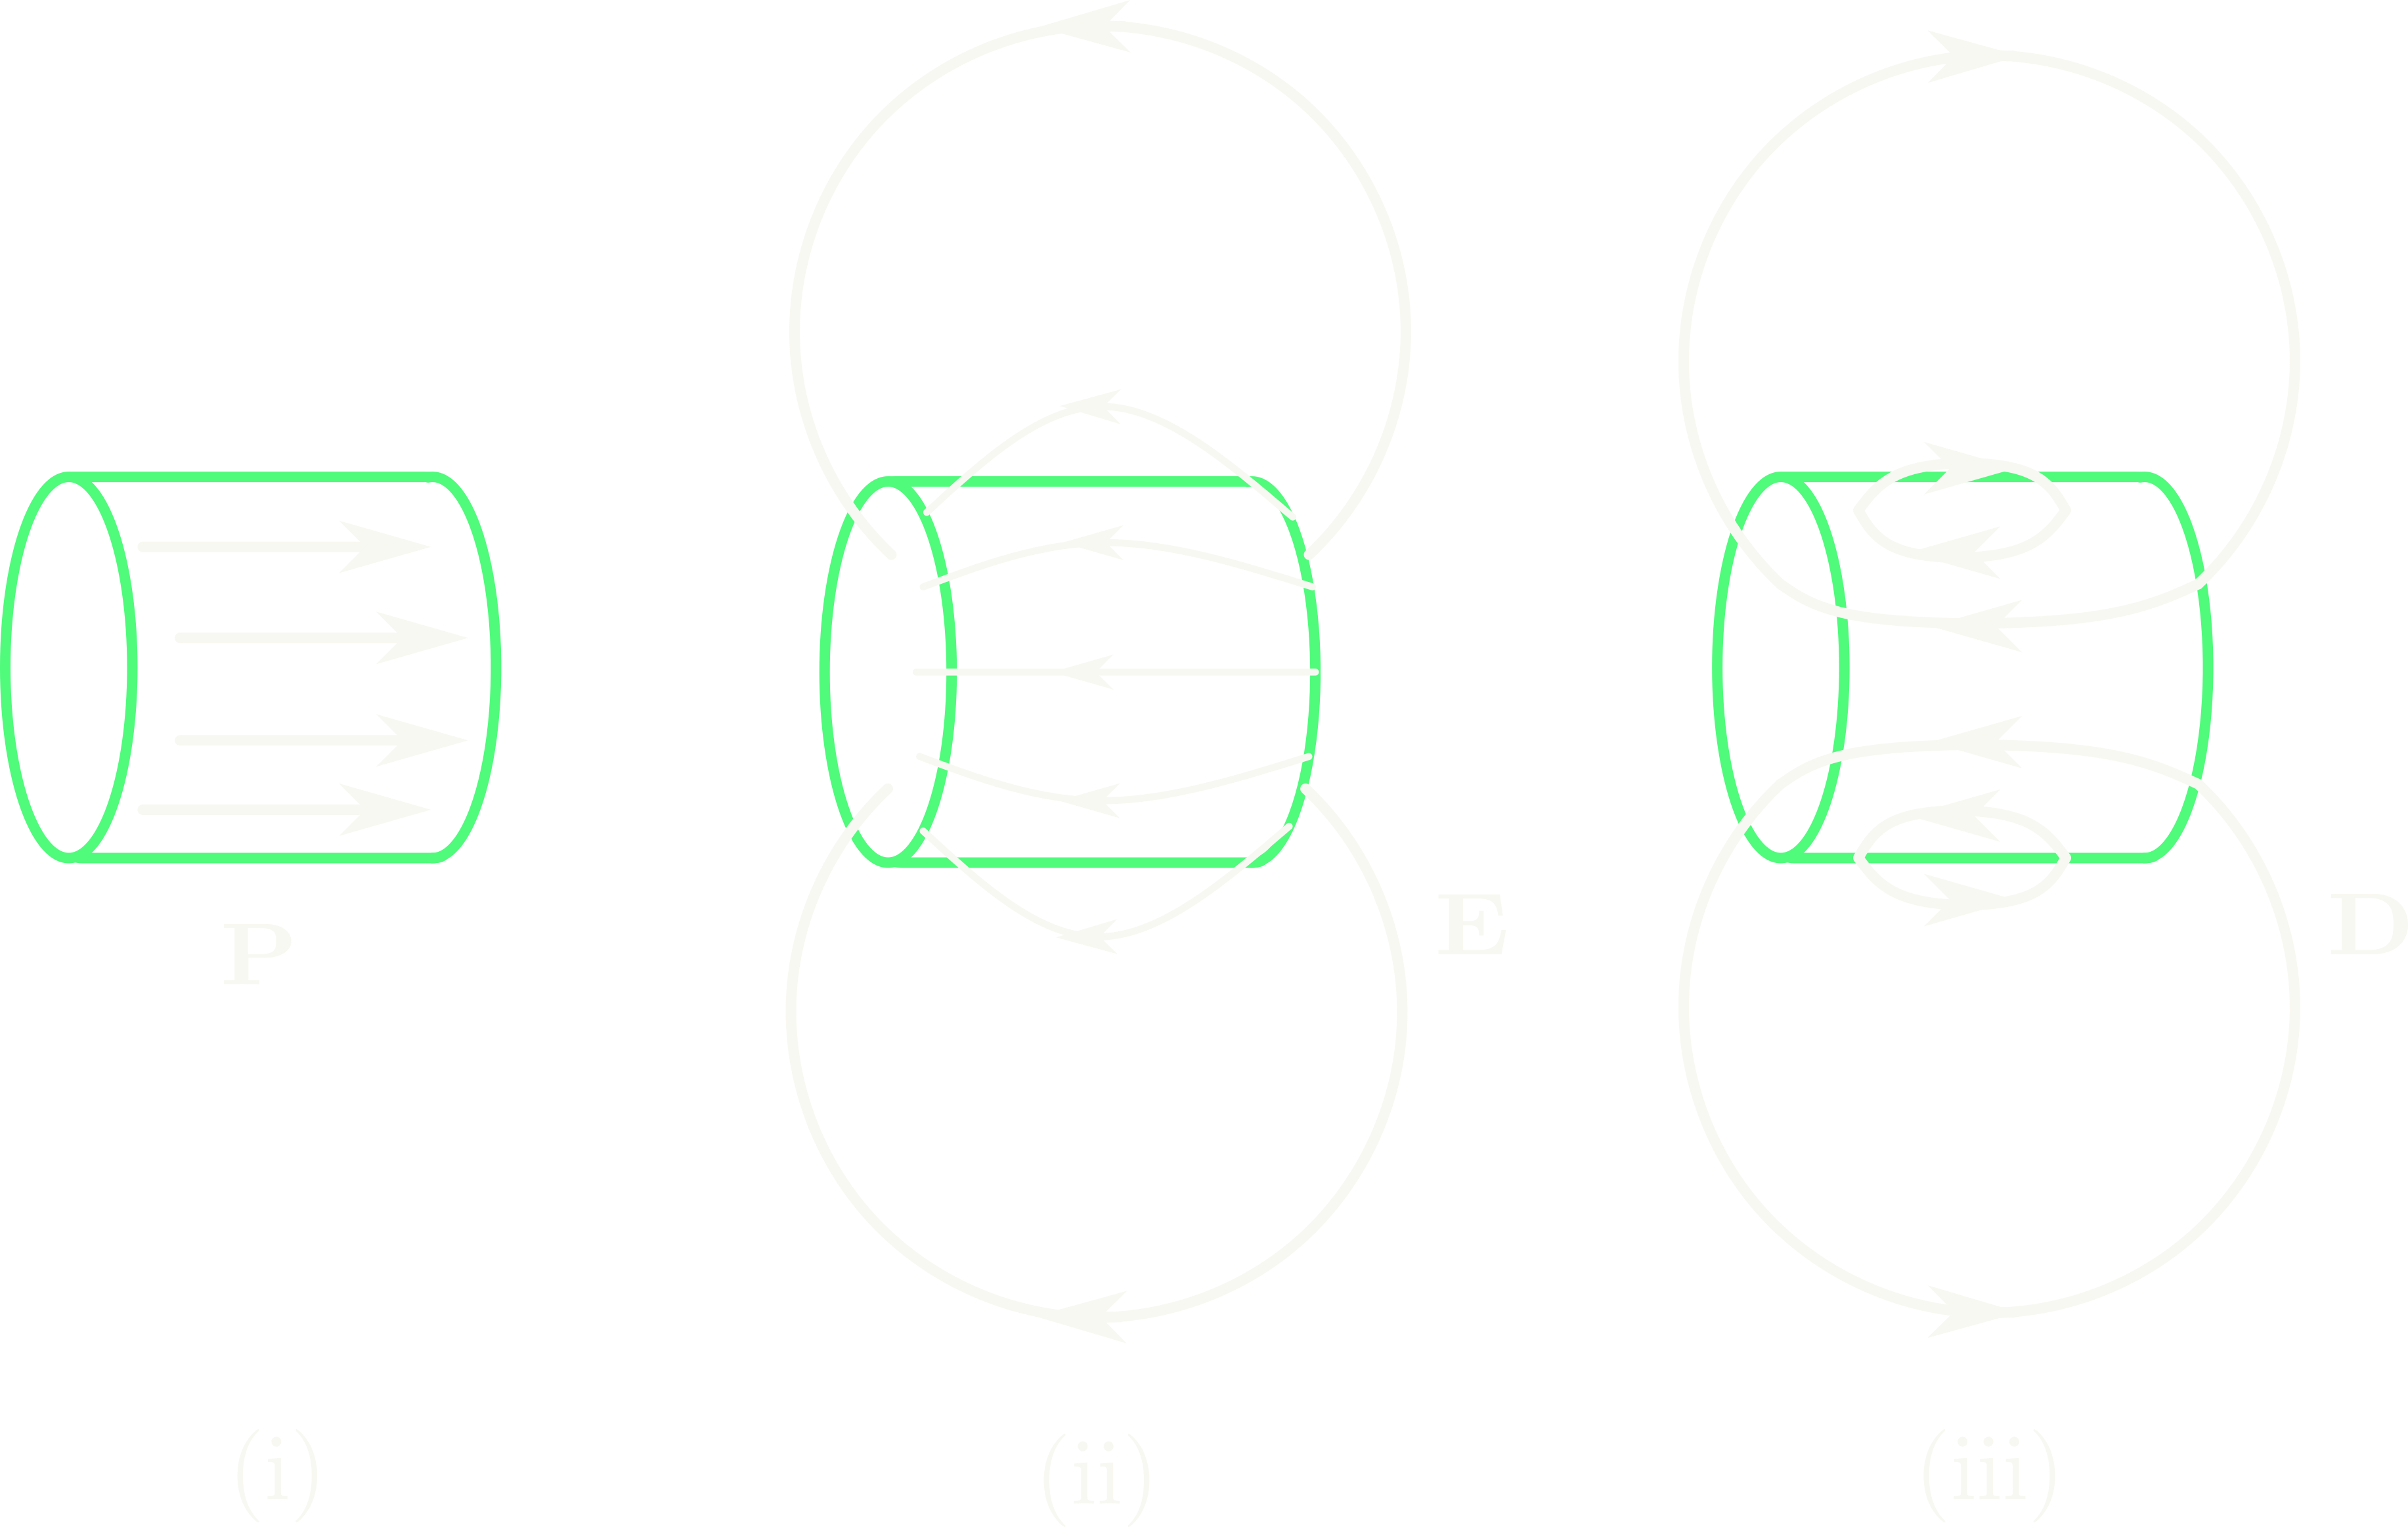
\includegraphics[width=0.8\linewidth]{hw7_1.png}
    \captionsetup{width=0.8\linewidth}
    \caption{Field lines for (i) $\vb P$ (ii) $\vb E$ (iii) $\vb D$}
    \label{fig:hw7_1}
\end{figure*}

\newpage
\paragraph{4.19} For a parallel plate capacitor, the E-field in the air between the plates is two times the E-field of a single plate
\begin{itemize}
    \item [(a)] \begin{align*}
        \vb E_\text{air} = 2\vb E_\text{plate} = \frac{\sigma}{\epsilon_0} \vu n
    \end{align*}
    where $\sigma = \pm Q/A$ is the surface charge density on the plates. The displacement field is
    \begin{align*}
        \oint D \vdot \dd{\vb a} &= Q_\text{free} \\
        D (A) &= \sigma A \\
        \implies D &= \sigma
    \end{align*}
    In the linear dielectric medium, $\vb D$ is proportional to $\vb E$ by
    \begin{align*} \tag{4.32} \label{eq:4.32}
        \vb D = \epsilon \vb E
    \end{align*}
    So
    \begin{align*}
        \implies E = \frac{D}{\epsilon} = \frac{\sigma}{\epsilon}
    \end{align*}
    and the potential difference between the plates is the sum of the potential differences in the air and the dielectric
    \begin{align*}
        V &= E d \\
        &= E_\text{air} d_\text{air} + E_\text{die} d_\text{die} \\
        &= \frac{\sigma}{\epsilon_0} \frac{d}{2} + \frac{\sigma}{\epsilon} \frac{d}{2} \qusing \sigma = \frac{Q}{A} \\
        &= \frac{Qd}{2A\epsilon_0} \qt[1 + \frac{\epsilon_0}{\epsilon}] \\
    \end{align*}
    Finally the capacitance of the half filled capacitor (a) is
    \begin{align*}
        C_a = \frac{Q}{V} = \frac{2A\epsilon_0}{d} \frac{1}{1 + \frac{\epsilon_0}{\epsilon}}
    \end{align*}
    Compared to the capacitance of a fully filled capacitor
    \begin{align*} \tag{2.54} \label{eq:2.54}
        C = \frac{A\epsilon_0}{d} 
    \end{align*}
    So the increase in capacitance is
    \begin{align*}
        \frac{C_a}{C} = \frac{2}{1 + \frac{\epsilon_0}{\epsilon}}
    \end{align*}
    Using the relative permittivity $\epsilon_r = \epsilon/\epsilon_0$, the capacitance of the half filled capacitor (a) increases by a factor of 
    \begin{align*}
        \boxed{
            \frac{C_a}{C} = \frac{2\epsilon_r}{1 + \epsilon_r}
        }
    \end{align*}
    \begin{itemize}
        \item [(i)] In air: the E-field increases by the same factor so for a given potential $V = Ed$,
        \begin{align*}
            \boxed{
                \vb E_\text{air} = \frac{2\epsilon_r}{1 + \epsilon_r} \frac{V}{d} \vu n
            }
        \end{align*}
        And since $\boxed{\vb P_\text{air} = 0}$ in air, the displacement field $\vb D = \epsilon_0 \vb E + \vb P$ is
        \begin{align*}
            \boxed{
                \vb D_\text{air} = \frac{2\epsilon_r}{1 + \epsilon_r} \epsilon_0 \frac{V}{d} \vu n
            }
        \end{align*}
        \item [(ii)] In the dielectric: The E-field in the dielectric is proportional to the E-field in the air (vacuum) by
        \begin{align*} \tag{4.35} \label{eq:4.35}
            \vb E = \frac{1}{\epsilon} \vb D = \frac{1}{\epsilon_r} \vb E_\text{vac}
        \end{align*}
        so
        \begin{align*}
            \boxed{
                \vb E_\text{die} = \frac{2}{1 + \epsilon_r} \frac{V}{d} \vu n
            }
        \end{align*}
        and from \eqref{eq:4.35}
        \begin{gather*}
            \vb D = \epsilon \vb E, \quad \epsilon = \epsilon_r \epsilon_0 \\
            \implies \boxed{
                \vb D_\text{die} = \frac{2\epsilon_r}{1 + \epsilon_r} \epsilon_0 \frac{V}{d} \vu n = \vb D_a
            }
        \end{gather*}
        Finally, we can find the polarization directly from either \eqref{eq:4.21} or 
        \begin{align*} \tag{4.30} \label{eq:4.30}
            \vb P = \epsilon_0 \chi_e \vb E = \epsilon_0 (\epsilon_r - 1) \vb E
        \end{align*}
        so we might as well use \eqref{eq:4.30} and get the polarization in the dielectric as 
        \begin{align*}
            \boxed{
                \vb P_\text{die} = \frac{2}{1 + \epsilon_r} \epsilon_0 (\epsilon_r - 1) \frac{V}{d} \vu n
            }
        \end{align*}
        \item [(iii)] The free bound surface charge is simply $\sigma_f = D$ so for the top plate
        \begin{align*}
            \boxed{
                \sigma_{f_\text{top}} = \frac{2\epsilon_r}{1 + \epsilon_r} \epsilon_0 \frac{V}{d}
            }
        \end{align*}
        and $\sigma_{f\text{bot}} = -\sigma_f$ for the bottom plate. And using $\sigma_b = \vb P \vdot \vu n$ where $\vu n$ points in the negative direction for the top plate, so
        \begin{align*}
            \boxed{
                \sigma_{b_\text{top}} = -\frac{2}{1 + \epsilon_r} \epsilon_0 (\epsilon_r - 1) \frac{V}{d} \quad \sigma_{b_\text{bot}} = -\sigma_{b\text{top}}
            }
        \end{align*}
    \end{itemize}
    \item [(b)] Again, from Gauss's law 
    \begin{gather*}
        E_\text{air} = \frac{\sigma_{f_\text{air}}}{\epsilon_0} \qand V = E_\text{air} d \\
        \implies \boxed{
            \sigma_{f_\text{air}} = \frac{\epsilon_0 V}{d}
        }
    \end{gather*}
    for the top plate ($-\sigma_{f_\text{air}}$ in the bottom plate) but in the dielectric, using $\vb D$
    \begin{align*}
        \oint \vb D \vdot \dd{\vb a} &= Q_\text{free} \\
        \implies D &= \sigma_{f_\text{die}}
    \end{align*}
    and from $D = \epsilon E_\text{die}$
    \begin{align*}
        E_\text{die} = \frac{\sigma_{f_\text{die}}}{\epsilon} = \frac{\sigma_f}{\epsilon_r \epsilon_0}
    \end{align*}
    Then using the potential difference $V = E_\text{die} d$
    \begin{align*}
        \implies \boxed{
            \sigma_{f_\text{die}} = \epsilon_r \epsilon_0 \frac{V}{d}
        }
    \end{align*}
    for the top plate (negative for bottom). From this, we can find the capacitance $C = Q/V$ where
    \begin{align*}
        Q &= \sigma_{f_\text{air}} \frac{A}{2} + \sigma_{f_\text{die}} \frac{A}{2} \\
        &= \frac{\epsilon_0 V A}{2d} + \frac{\epsilon_r \epsilon_0 V A}{2d} 
    \end{align*}
    so
    \begin{align*}
        \implies C &= \frac{A\epsilon_0}{2d} (1 + \epsilon_r)  
    \end{align*}
    From \eqref{eq:2.54}, the capacitance increases by a factor of
    \begin{align*}
        \boxed{
            \frac{C_b}{C} = \frac{1 + \epsilon_r}{2}
        }
    \end{align*}
    \begin{itemize}
        \item [(i)] The E-field in the air is just the E-field between two plates
        \begin{align*}
            \boxed{
                \vb E_\text{air} = \frac{V}{d} \vu n
            }
        \end{align*}
        and $\boxed{\vb P_\text{air} = 0}$ for air thus the displacement field \eqref{eq:4.21} $\vb D = \epsilon_0 \vb E + 0 $, or 
        \begin{align*}
            \boxed{
                \vb D_\text{air} = \epsilon_0 \frac{V}{d} \vu n
            }
        \end{align*}
        \item [(ii)] The E-field in the dielectric using \eqref{eq:4.32}:
        \begin{align*}
            \vb E_\text{die} = \frac{1}{\epsilon} \vb D
        \end{align*}
        where $D = \sigma_{f_\text{die}}$ so
        \begin{align*}
            \boxed{
                \vb D = \epsilon_r \epsilon_0 \frac{V}{d} \vu n
            }
        \end{align*}
        Then we can use $\epsilon = \epsilon_r \epsilon_0$ so
        \begin{align*}
            \boxed{
                \vb E_\text{die} = \frac{V}{d} \vu n = \vb E_\text{air}
            }
        \end{align*}
        Now the polarization is given by \eqref{eq:4.30}
        \begin{align*}
            \boxed{
                \vb P_\text{die} = \epsilon_0 (\epsilon_r - 1) \frac{V}{d} \vu n
            }
        \end{align*}
        Finally, the bound charge is $\sigma_b = \vb P \vdot \vu n$ so
        \begin{align*}
            \boxed{
                \sigma_{b_\text{top}} = -\epsilon_0 (\epsilon_r - 1) \frac{V}{d} \quad \sigma_{b_\text{bot}} = -\sigma_{b_\text{top}}
            }
        \end{align*}
    \end{itemize}
\end{itemize}

\newpage
\paragraph{4.37} Between two linear dielectric, show that the E-field lines bend by
\begin{align*} \tag{4.68} \label{eq:4.68}
    \frac{\tan\theta_2}{\tan\theta_1} = \frac{\epsilon_2}{\epsilon_1}
\end{align*}
Since $\sigma_f = 0$ so from the boundary conditions 
\begin{align*}
    D^\perp_1 - D^\perp_2 &= \sigma_b = 0 \implies D^\perp_1 = D^\perp_2
\end{align*}
or from \eqref{eq:4.32}
\begin{align*}
    D_{y_1} = D_{y_2} \implies \epsilon_1 E_{y_1} = \epsilon_2 E_{y_2}
\end{align*}
Also from the boundary conditions, the parallel components of $\vb E$ are continuous so
\begin{align*}
    E_{x_1} = E_{x_2} \implies \tan\theta_1 = \frac{E_{y_1}}{E_{x_1}},\qand \tan\theta_2 = \frac{E_{y_2}}{E_{x_2}}
\end{align*}
Thus
\begin{align*}
    \frac{\tan\theta_2}{\tan\theta_1} &= \frac{E_{y_2}/E_{x_2}}{E_{y_1}/E_{x_1}} \\
    &= \frac{E_{y_2}}{E_{y_1}} \qusing E_{y_1} = \frac{\epsilon_2}{\epsilon_1} E_{y_2} \\
    \frac{\tan\theta_2}{\tan\theta_1} &= \frac{\epsilon_2}{\epsilon_1}
\end{align*}
From Snell's Law
\begin{align*}
    n_1 \sin\theta_1 = n_2 \sin\theta_2
\end{align*}
where a convex lens has $n_2 > n_1$ which makes the angle of refraction smaller than the angle of incidence $\theta_2 < \theta_1$ thus the light ray bends towards the normal or ``focuses'' the light.
For the dielectric interface, its convex lens
\begin{align*}
    \epsilon_2 > \epsilon_1 \implies \tan\theta_2 > \tan\theta_1
\end{align*}
So $\theta_2 > \theta_1$, thus the E-field lines bend away from the normal which will ``defocus'' the E-field.

\end{document}